%%%%%%%%%%%%%%%%%%%%%%%%%packages%%%%%%%%%%%%%%%%%%%%%%%%%%%
\documentclass[a4paper,12pt,titlepage]{article}
\usepackage[francais]{babel}
\usepackage[utf8]{inputenc}
\usepackage[pdftex]{graphicx}
\usepackage{vmargin}
\usepackage{fancyhdr}
\usepackage{lastpage}
\usepackage{color}
\usepackage{xcolor}
\definecolor{LightGray}{gray}{0.7}
\usepackage{minted}
\usepackage{titlesec}
\usepackage{circuitikz}
 \usepackage{siunitx}


%%%%%%%%%%%%%%%%%%%%%%%%%%%%%%%%%%%%%%%%%%%%%%%%%%%%%%%%%%%%
\pagestyle{fancy}
\renewcommand{\headrulewidth}{0.2pt}
\renewcommand{\footrulewidth}{0.2pt}

\title{
    
\includegraphics[width=0.15\textwidth]{../logos/UM.png}
    \hspace{1cm}    
    
\includegraphics[width=0.4\textwidth]{../logos/Polytech.png}\\
    \vspace{5cm}
    \textbf{T.P.\\Électronique}\\ TEYSSIER Maxime\\
    \vfill
}
\begin{document}
\cfoot{Pages \thepage/\pageref{LastPage}}
\lhead{TEYSSIER Maxime}
\rhead{EII Systèmes Embarqués 3}
\rfoot{Polytech' Montpellier}
\lfoot{UM}
\maketitle
\newpage
%%%%%%%%%%%%%%%%%%%%%%%%%%%%%%%%%%%%%%%%%%%%%%%%%%%%%%%%%%%%%%

\begin{center}
    \Large{Exercices d'entraînement de Pspice}
\end{center}
\section{Exercice 1}

Nous souhaitons connaitre le potentiel en continu en \textit{s} quand e$_1$=1V, e$_2$=2CV, I=1mA.
\textit{s} étant la tension de R$_4$.\\
Nous avons:R1 = 3,3 k$\Omega$ ; R2 = 6,8 k$\Omega$ ; R3 = 4,7 k$\Omega$ ; R4 = 2,2 k$\Omega$.\\

\begin{center}
    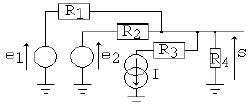
\includegraphics[width=0.4\textwidth]{Exo1/Exo1.PNG}\\
    \textit{Circuit exercice 1}\\
\end{center}

Deux sources de tension et une source de courant sont présentes dans le circuit, pour cela nous allons calculer chaque valeur de \textit{s} pour $e_1$, $e_2$, I.

\subsubsection{e$_1$ actif, autres sources inutilisées}

Pour pouvoir connaître le potentiel de \textit{s} avec $e_1$ actif seulement, nous allons faire un court-circuit sur $e_2$ et I.
Donc $e_2$ devient un simple fil, I et R$_3$ sont supprimés. 

\begin{center}
    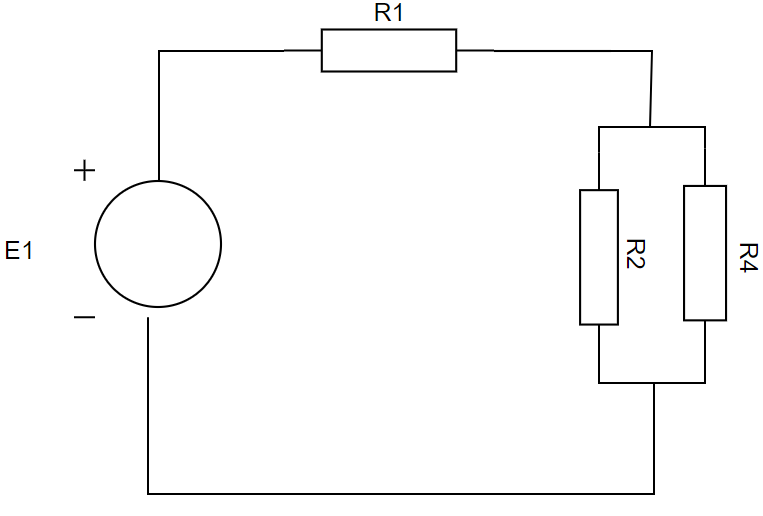
\includegraphics[width=0.4\textwidth]{Exo1/Exo1-1.PNG}\\
    \textit{Court-circuit de $e_2$ et I}\\
\end{center}

Nous pouvons remarquer un pont diviseur de tension sur ce circuit, cela dit nous avons deux résistances en parallèles. Nous devons pour ce pont diviseur faire une résistance équivalente entre R$_2$ et R$_4$. Ce pont diviseur nous donnera la valeur de la tension de R4 (soit U$_{R_4}$). On pose:\\

\begin{center}
    $s_1 = U_{R_4} = e_1 \frac{\frac{R_2R_4}{R_2+R_4}}{R_1+\frac{R_2R_4}{R_2+R_4}} = \frac{1.66}{3.3+1.66} = 0.335$V 
\end{center}

La valeur de $s_1$ (écrit "$s_1$" car nous allons calculer 3 fois la valeur de \textit{s}) est de 0.335 Volts

\subsection{Théorie}

\subsubsection{$e_2$ actif, autres sources inutilisées}

Pour pouvoir connaître le potentiel de \textit{s} avec $e_2$ actif seulement, nous allons faire un court-circuit sur $e_2$ et I.
Donc  $e_1$ devient un simple fil, I et R$_3$ est supprimé. 

\begin{center}
    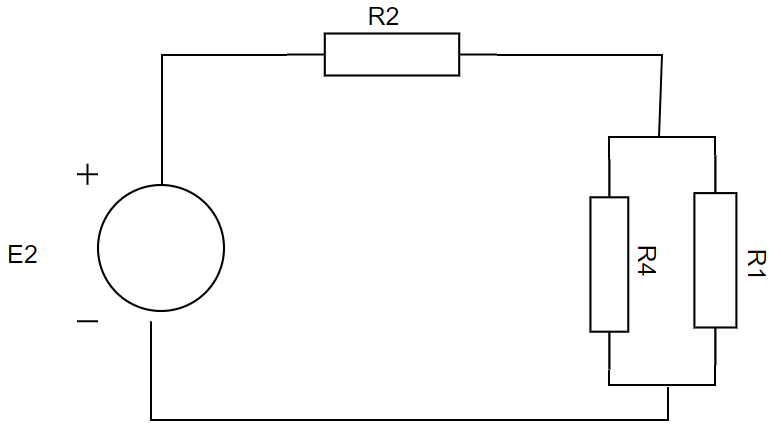
\includegraphics[width=0.4\textwidth]{Exo1/Exo1-2.PNG}\\
    \textit{Court-circuit de $e_1$ et I}\\
\end{center}

Comme précédemment nous remarquons un pont diviseur. Nous allons poser la même forme de calcul:\\


\begin{center}
    $s_2 = U_{R_4} = e_2 \frac{\frac{R_1R_4}{R_1+R_4}}{R_2+\frac{R_1R_4}{R_1+R_4}} = \frac{1.66}{3.3+1.66} = 0.325$V 
\end{center}

La valeur de $s_2$ est de 0.325 Volts

\subsubsection{\textit{I} actif, autres sources inutilisées}
Pour pouvoir connaître le potentiel de \textit{s} avec $e_2$ actif seulement, nous allons faire un court-circuit sur $e_1$ et $e_2$.
Donc  $e_1$ et , $e_2$ deviennent de simple fil.\\

\begin{center}
    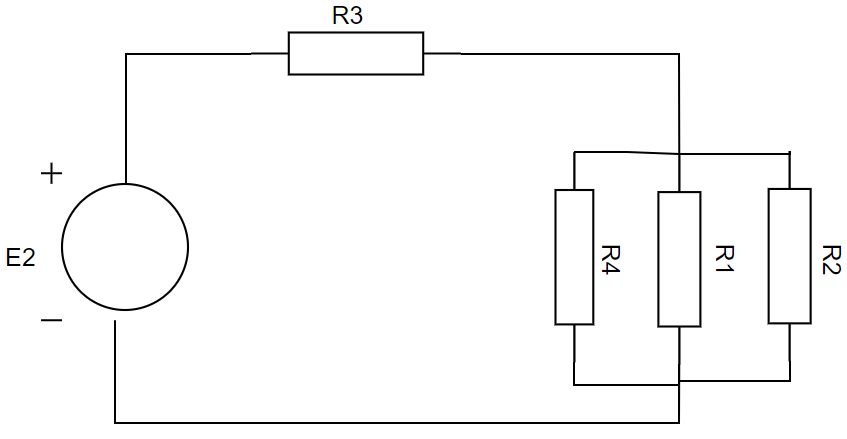
\includegraphics[width=0.4\textwidth]{Exo1/Exo1-3.PNG}\\
    \textit{Court-circuit de $e_1$ et $e_2$}
\end{center}

Nous avons comme données sur ce circuit: $I, R_1, R_2, R_4$. Nous pouvons de cela, faire une résistance équivalente $R_{124}$ avec $R_1, R_2, R_4$ pour pouvoir appliquer la loi d'Ohm: $U_{R_{124}}$ = -I\times $R_{124}$. \newline On pose:\\

\begin{center}
$R_{eq_{24}} = \frac{R_2R_4}{R_2+R_4} = \frac{6.8\times2.2\times10^6}{9\times10^3} = 1.66\times10^3\Omega$\\

$R_{eq_{124}} = \frac{R_1R_24}{R_1+R_24} = \frac{3.3\times1.66\times10^6}{(3.3+1.66)\times10^3} = 1.1\times10^3\Omega$\\

$s_3 = U_{R_{124}= -I\times R_{124} = -0.001\times1100 = }\SI{-1.1}{\volt}$\\
\end{center}
La valeur de s3 est de -1.1 Volts
\subsubsection{Résultat de \textit{s}}


Maintenant que nous avons tout les résultats de \textit{s} nous allons pouvoir les additionnés pour avoir le résultats dans le circuit complet. On pose:\\

\begin{center}
$s = s_1 + s_2 + s_3 = 0.335 + 0.325 + (-1.1) \approx$ \SI{-0.44}{\volt}
\end{center}

\subsection{Simulation}

Nous allons créer sur l'outil Pspice simuler le circuit pour interpréter le résultat qui ressort et le comparer avec le résultat théorique.  
\subsubsection{Création du fichier \textit{.cir}}

\begin{minted}[
    baselinestretch=1.4,
    bgcolor=LightGray,
    fontsize=\footnotesize]
{php}
Exercice1
* fichier exo 1.cir
V1 1 0 DC=1; Création d une source de tension
V2 2 0 DC=2; Création d une source de tension
I1  3 0 1m; Création d une source de courant
R1 1 4 3.3k; Création d une résistance
R3 3 4 4.7k; Création d une résistance
R2 2 4 6.8k; Création d une résistance
R4 4 0 2.2k, Création d une résistance
.OP; Calcul des tensions et courant de repos
.END
\end{minted}

\subsubsection{Résultat de la simulation dans le fichier .out}
\begin{minted}[
    baselinestretch=1.4,
    bgcolor=LightGray,
    fontsize=\footnotesize]
{php}
 NODE   VOLTAGE     NODE   VOLTAGE     NODE   VOLTAGE     NODE   VOLTAGE

(    1)    1.0000  (    2)    2.0000  (    3)   -5.1453  (    4)    -.4453  

    VOLTAGE SOURCE CURRENTS
    NAME         CURRENT

    V1          -4.380E-04
    V2          -3.596E-04

    TOTAL POWER DISSIPATION   1.16E-03  WATTS
\end{minted}

\subsection{Conclusion}

La simulation dans l'outil Pspice nous a donné pour le noeud 4 un résultat de \textit{-.4453}. Ce résultat est équivalent au notre. Le notre n'est pas si précis car nous avons arrondit sur nos résultat, cela dit nous sommes très proche. Nous pouvons conclure que le résultat de \textit{s} est de \SI{-0.4453}{\volt}

\section{Exercice 2}
On désire connaître la résistance équivalente entre les noeuds A et B.

\begin{center}
    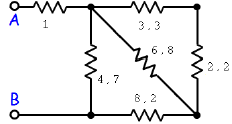
\includegraphics[width=0.4\textwidth]{Exo2/Exo2.PNG}\\
    \textit{Circuit exercice 2}\\
\end{center}

\subsection{Théorie}

Pour calculer la résistance équivalent, on pose: 
\begin{center}
    $R_{eq} = 1+\frac{4.7\times(\frac{6.8\times(3.3+2.2)}{6.8+(3.3+2.2)}+8.2)}{4.7+(\frac{6.8\times(3.3+2.2)}{6.8+(3.3+2.2)}+8.2)} \approx 4.3\Omega$
\end{center}

\subsection{Simulation}
\subsubsection{Création du fichier \textit{.cir}}
\begin{minted}[
    baselinestretch=1.4,
    bgcolor=LightGray,
    fontsize=\footnotesize]
{php}
Exercice2
* Exercice 2
V1 0 1 DC=1; Gen tension
R1 1 2 1; Res
R2 2 3 3.3; Res 
R3 3 4 2.2; Res
R4 2 4 6.8; Res
R5 4 0 8.2; Res
R6 2 0 4.7; Res
.OP; Calcul tension/courant
.END
\end{minted}
\subsubsection{Résultat de la simulation dans le fichier .out}
\begin{minted}[
    baselinestretch=1.4,
    bgcolor=LightGray,
    fontsize=\footnotesize]
{php}
 NODE   VOLTAGE     NODE   VOLTAGE     NODE   VOLTAGE     NODE   VOLTAGE

(    1)   -1.0000  (    2)    -.7682  (    3)    -.6435  (    4)    -.5604  

    VOLTAGE SOURCE CURRENTS
    NAME         CURRENT

    V1          -2.318E-01

    TOTAL POWER DISSIPATION   2.32E-01  WATTS
\end{minted}

Les valeurs disponibles sur Pspice après simulation sont la tension et le courant. Pour cela nous avons qu'à utiliser la loi d'Ohm pour retrouver la résistance équivalente. On pose: 
\begin{center}
U = RI\\

$R = \frac{U}{I} = \frac{1}{0.318} \approx 4.3\Omega$
\end{center}

\subsection{Conclusion}

Nous pouvons en conclure que Pspice nous retourne les valeurs cohérentes par rapport à notre théorie.\\

\section{Exercice 3}

On désire savoir dans quelle plage ce circuit est assimilable à un dérivateur.\\

\begin{center}
    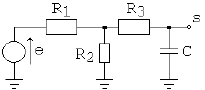
\includegraphics[width=0.4\textwidth]{Exo3/Exo3.PNG}\\
    \textit{Circuit exercice 3}\\
\end{center}
On donne R = 4,7 kΩ ; C = 2,2 nF.\\


\subsection{Théorie}\\

Nous allons dans un premier temps représenter le circuit différemment, nous appliquons le théorème de Thévenin: 
\begin{center}
    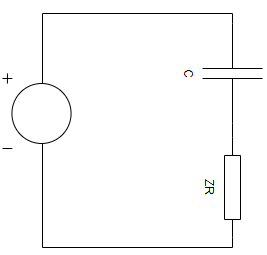
\includegraphics[width=0.4\textwidth]{Exo3/Exo3(bis).PNG}\\
    \textit{Circuit modifier}\\
\end{center}

Nous posons: 

\begin{center}
    $Z_e = \frac{1}{j\omega c}$\\
    $Z_e = R$\\
    $\tau = RC$\\
    $H(j\omega) = \frac{\underline{s}}{\underline{z}} = \frac{Z_R}{Z_R+Z_e} = \frac{R}{R+\frac{1}{j\omega c}} = \frac{1}{1+\frac{1}{RCj\omega}} =  \frac{1}{1+\frac{1}{\tau j\omega}}$
\end{center}

\begin{itemize}
    \item Quand $\omega$  $\to$ $\infty$, H(j$\omega$) $\approx$ 1 car on pose:
    \begin{center}
        20log($|$Hj$\omega$)$|$) = 20log(1)=0\\
        
        $|H(j\omega)| = e^0$=1\\
    \end{center}\\
    \item Nous avons une asymptote à 0dB/décade\\
    \item Quand $\omega \to 0$, H(j$\omega$)$\approx \tau j\omega$\\
    \begin{center}
        H(j$\omega$) = $\frac{1}{1+\frac{1}{\tau j \omega}} = \frac{\tau j\omega}{1+\tau j \omega} $\\
        Vu que $\tau \to$ 0 :\\
        H(j$\omega$) = $\frac{0}{1+0}=0$
    \end{center}\\
    \item Le dénominateur peu négliger le 1 car $\tau$ étant en numérateur (de plus que le dénominateur) il régit le calcul. On pose:
    \begin{center}
        $20log(|H(10\omega j)|)$ = 20 log(10)+20log($\omega j$)
    \end{center}\\
    \item 20log(10) = 20. Nous pouvons alors en déduire une asymptote à 20dB/décade.
    \item La fréquence ce calcul via: 
    \begin{center}
        $\tau = RC = 4.7\times10^3\times2.2\times10^{-9} = 10.34\times10^{-6}$\\
        $F_0 = \frac{w}{2\pi} = \frac{1}{2\pi\tau} = \frac{1}{2\pi\times10.34\times10^{-6}} = 15392.16$\\
    \end{center}
    \item En $F_0$, on pose: 
    \begin{center}
        H = $\frac{1}{1+\frac{1}{j}} = \frac{j}{j+i}$\\
        $20log(|H|) = 20log(\frac{|j|}{|j+i|}) = 20log(|j|)-20log(|i|) = 0-20log(\sqrt{2}) \approx -3$
    \end{center}
\end{itemize}

\subsection{Simulation}
\subsubsection{Création fichier .cir}
\begin{minted}[
    baselinestretch=1.4,
    bgcolor=LightGray,
    fontsize=\footnotesize]
{php}
Exercice3
* Exercice 3
Ve 1 0 AC=1
R1 2 0 4.7k
C1 1 2 2.2n
.AC DEC 1000 100 100k
.PROBE
.END
\end{minted}
\subsubsection{Résultat de la simulation dans le fichier .out}
\begin{center}
    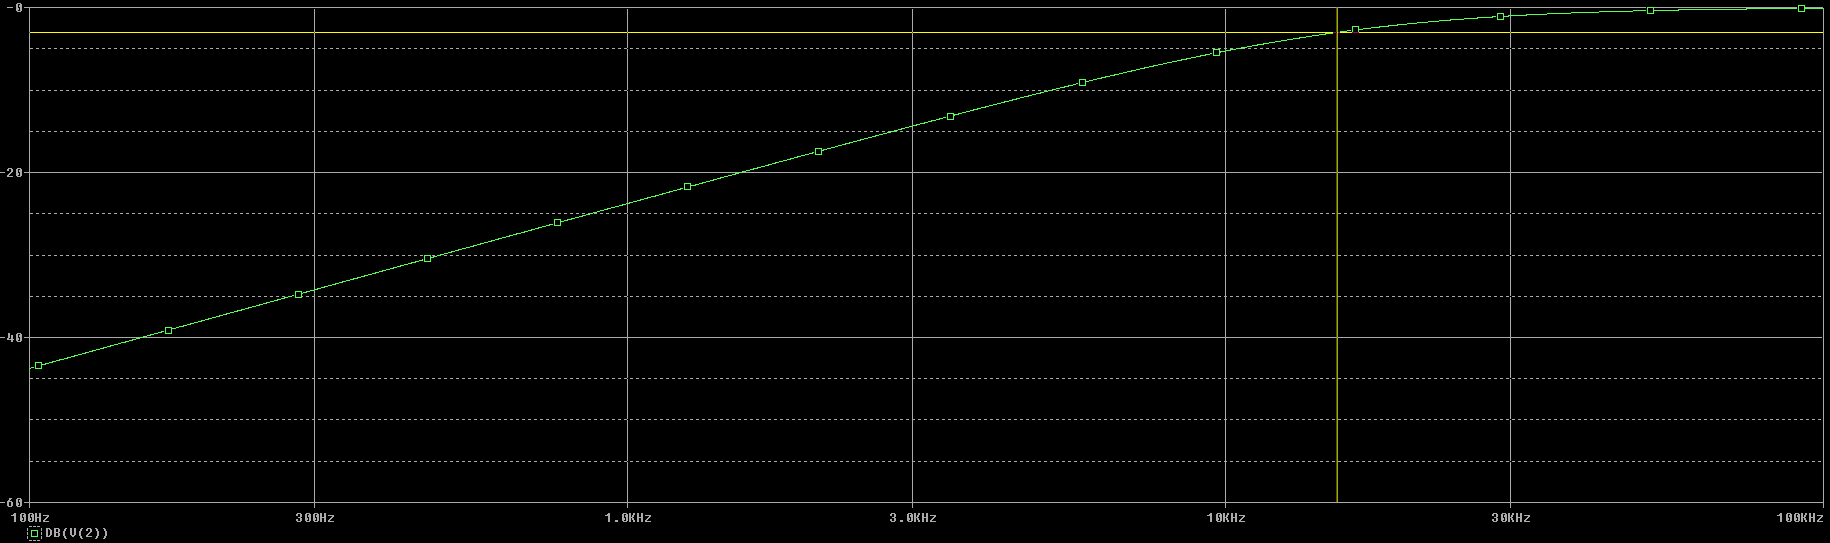
\includegraphics[width=\textwidth]{Exo3/Exo3-1.PNG}\\
    \textit{Courbe : dB(V(2))}\\
    \vspace{0.5cm}
    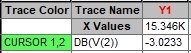
\includegraphics[witdh=0.4\textwidth]{Exo3/Exo3-1(bis).PNG}\\
    \textit{Résultat sur le tableur}
\end{center}

\subsection{Conclusion}
Nous pouvons conclure qu'avec la simulation, nous avons bien trouvé -3dB avec le curseur pour la fréquence de coupure de F$_0 \approx$ 15,3kHz.

\section{Exercice 4}
Dans le but de calculer la forme d'onde s(t) quand e(t) est un échelon de tension d'amplitude E$_0$ = $\SI{3}{\volt}$ On donne R$_1$ = 3,3 k$\Omega$ ; R$_2$ = 6,8 k$\Omega$ ; R$_3$ = 4,7 k$\Omega$ ; C = 100 μF.
\begin{center}
    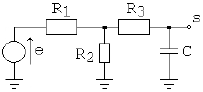
\includegraphics[width=0.4\textwidth]{Exo4/Exo4.PNG}\\
    \textit{Circuit exercice 4}
\end{center}
\subsection{Théorie}
Sur ce circuit nous allons appliquer le théorème de Thévenin pour simplifier:\\
\begin{center}
    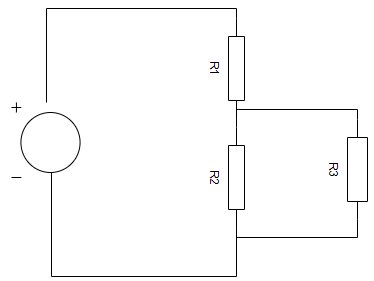
\includegraphics[width=0.4\textwidth]{Exo4/Exo4-1.PNG}\\
    \textit{Circuit avec application Thévenin (1)}
\end{center}

Maintenant nous remarquons un pont diviseur, ce qui donne:

\begin{center}
    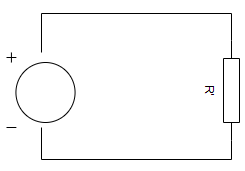
\includegraphics[width=0.4\textwidth]{Exo4/Exo4-2.PNG}\\
    \textit{Application de pont diviseur(2)}
\end{center}

\begin{itemize}
    \item Notre tension à vide est: 
        \begin{center}
            $e'=e\times\frac{R_2}{R_1+R_2}$
        \end{center}
    \item Pour calculer R', nous avons besoin de connaître l'intensité de court-circuit. On pose (via schéma (1)):
        \begin{center}
            U$_3$ = $e'\times\frac{R_{23}}{R_1+R23}$\\
            $I_{cc} = \frac{U_3}{R_3} = e'\times\frac{R_{23}}{R_3\times(R_1+R23)}$
            R'=$\frac{e'}{I_{cc}} = \frac{R_3\times(R_1+R_{23})}{R_{23}}$
        \end{center}
\end{itemize}

De ce fait, le circuit devient: 
\begin{center}
    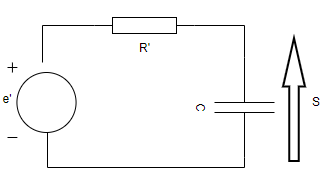
\includegraphics[width=0.4\textwidth]{Exo4/Exo4-3.PNG}\\
\end{center}
On peut alors poser: 
\begin{center}
    $e'(t) = R'\times I + s(t) = R'\times C\frac{ds}{dt} + s(t) $
\end{center}

\subsection{Simulation}
\subsubsection{Création fichier .cir}
\begin{minted}[
    baselinestretch=1.4,
    bgcolor=LightGray,
    fontsize=\footnotesize]
{bash}
V1 1 0 pulse (0 3 2m 0 0 2 2)
R1 1 2 3.3k
R2 2 0 6.8k
R3 2 3 4.7k
C1 3 0 100u
.TRAN 8m 8
.PROBE
.END
\end{minted}
\subsubsection{Résultat de la simulation dans le fichier .out}
\begin{center}
    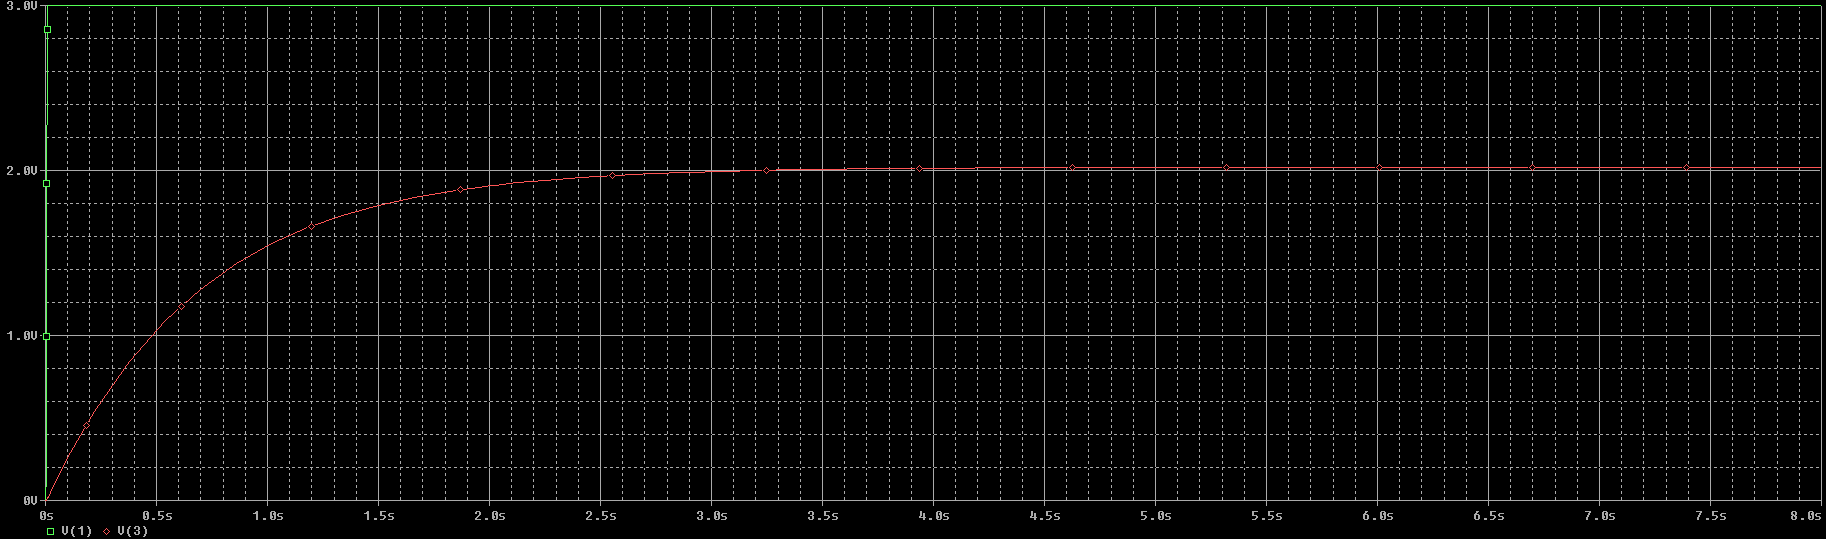
\includegraphics[width=\textwidth]{Exo4/Exo4-4.PNG}
\end{center}
\subsection{Conclusion}

Nous pouvons remarquer que la tension de V(3) tend vers 2V.

\section{Exercice 5}
Le but étant de connaître s(t) en régime établi.
\begin{center}
    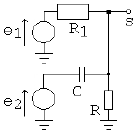
\includegraphics[width=0.4\textwidth]{Exo5-6/Exo5.PNG}\\
\end{center}
\subsection{Fichier .cir}
\begin{minted}[
    baselinestretch=1.4,
    bgcolor=LightGray,
    fontsize=\footnotesize]
{php}
Exercice5
* Execrice 5
V1 0 1 DC=2
V2 2 0 sin(0 1 30k 0 0)
R1 1 3 4.7k
R  3 0 4.7k
C  2 3 2.2n
.TRAN 10n 400u 0 10n
.PROBE
.END
\end{minted}
\subsection{Simulation}
\begin{center}
    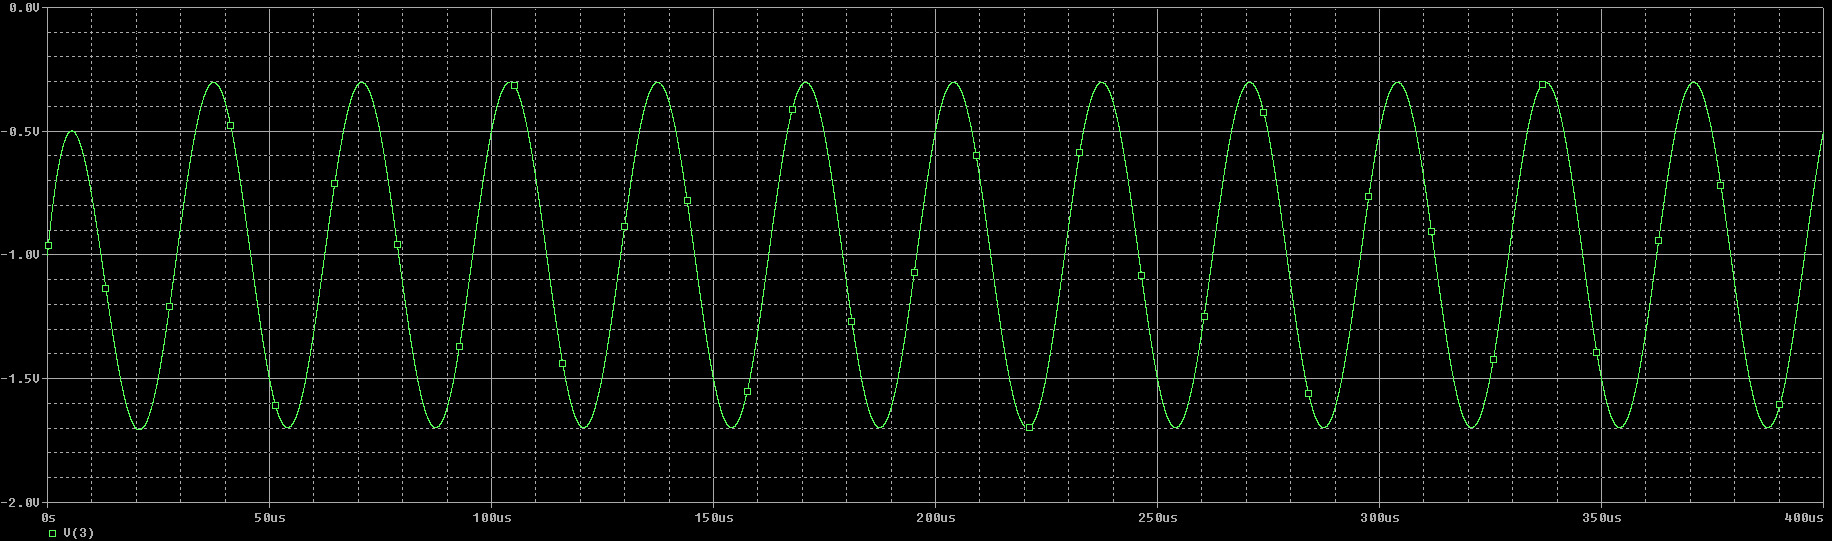
\includegraphics[width=\textwidth]{Exo5-6/Exo5-1.PNG}\\
    \textit{Résultat de la simulation}
\end{center}

\section{Exercice 6}
Le but est de donner f$_0$, (= $\omega$0/2$\pi$) sa fréquence propre sans amortissement,
z, son coefficient d’amortissement réduit, f$_R$, sa fréquence de résonance.
\begin{center}
    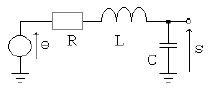
\includegraphics[width=0.4\textwidth]{Exo5-6/Exo6.PNG}\\
\end{center}

\subsection{Simulation}
\begin{minted}[
    baselinestretch=1.4,
    bgcolor=LightGray,
    fontsize=\footnotesize]
{php}
Exercice6
* Exercice 6

Ve 1 0 PULSE(-1 1 0 30u 30u 20u 100u)
R1 1 2 500
L1 2 3 200m
C1 3 0 1.2665n
.TRAN 10n 5m 0 10n
.PROBE
.END
\end{minted}

\begin{center}
    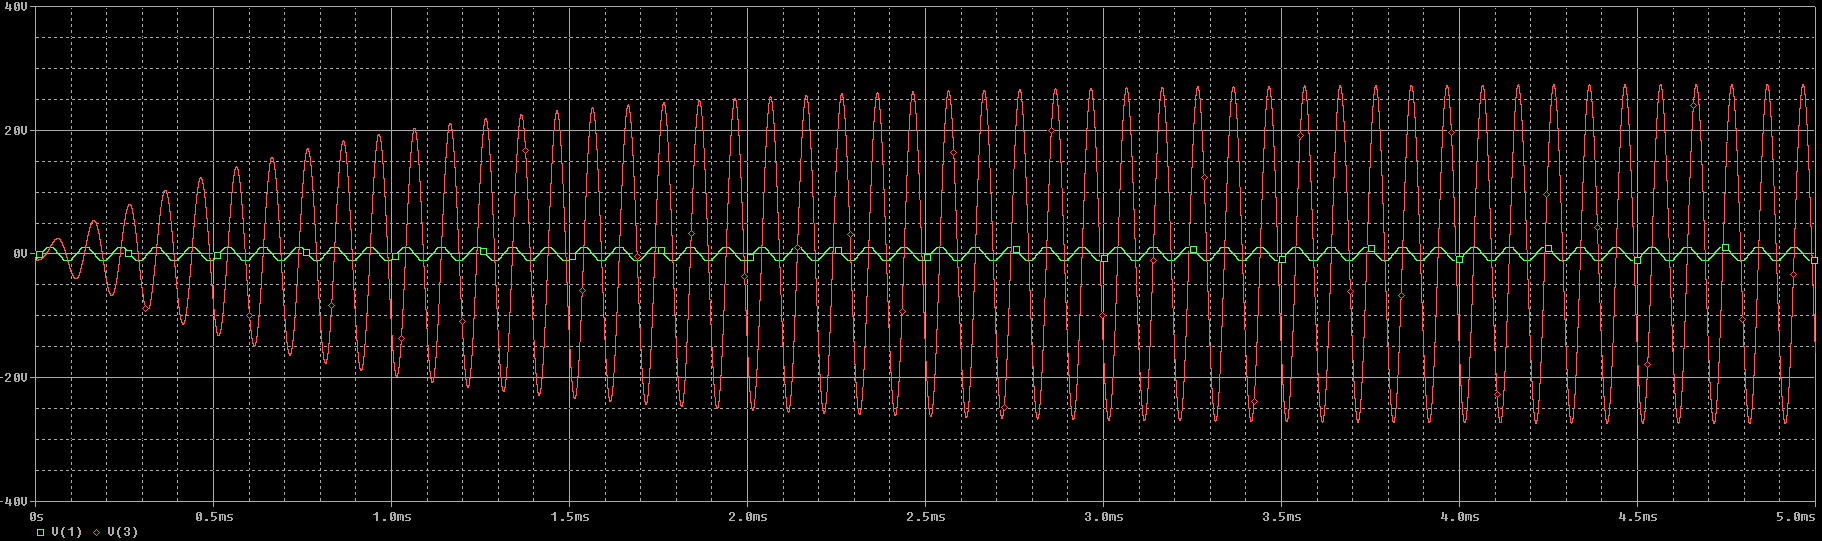
\includegraphics[width=\textwidth]{Exo5-6/Exo6-1.PNG}
\end{center}

\end{document}